\documentclass[twocolumn]{article}
%\usepackage[spanish]{babel}
\usepackage[utf8]{inputenc}
\usepackage{amsmath}
\usepackage{natbib}
\usepackage{microtype}
\usepackage{etoolbox}
\usepackage{amssymb}
\usepackage{graphicx}
\usepackage{lipsum}
\usepackage{fancyhdr}
\usepackage{abstract}
\usepackage{geometry}
\usepackage{booktabs}
%Ubicacion de los graficos 
\graphicspath{ {imagenes/} }

% DEFINIR LOS COMANDOS QUE FALTAN
\providecommand{\apjs}{ApJ Suppl. Ser.}
\providecommand{\aj}{Astron. J.}
\providecommand{\apj}{Astrophys. J.}
\providecommand{\apjl}{Astrophys. J. Lett.}
\providecommand{\aap}{Astron. Astrophys.}
\providecommand{\mnras}{Mon. Not. R. Astron. Soc.}
\providecommand{\pasa}{Publications of the Astronomical Society of Australia}
% Configuración de página
\geometry{a4paper, margin=1in}

% Configuración de encabezados
\pagestyle{fancy}
\fancyhf{}
\fancyhead[L]{\small Morfología y propiedades de galaxias en Sloan}
\fancyhead[R]{\small \thepage}
\fancyfoot[C]{\footnotesize Astronomía Extragaláctica - 2025 - J.M. Puddu }

% Configuración del abstract para una columna
\renewcommand{\abstractname}{Abstract}
\setlength{\absleftindent}{0pt}
\setlength{\absrightindent}{0pt}

\title{Morfología y propiedades de galaxias en Sloan}
\author{J.M. Puddu \\ FAMAF - Universidad Nacional de Córdoba - Argentina}

\begin{document}

\twocolumn[
\begin{@twocolumnfalse}
    \maketitle
    \begin{abstract}
        \noindent Este trabajo presenta una implementación computacional de métodos estadísticos para el análisis de la morfología y propiedades de galaxias utilizando datos del Sloan Digital Sky Survey (SDSS). Se estudian las características visuales y espectroscópicas de galaxias con el objetivo de comprender los procesos físicos subyacentes y extraer información relevante para estudios extragalácticos.
        
        \vspace{0.5em}
        \noindent\textbf{Palabras clave}: Galaxias, Morfología, SDSS, Astronomía extragaláctica, Análisis estadístico
    \end{abstract}
    \vspace{2em} % Espacio después del abstract
\end{@twocolumnfalse}
]

\section{Introducción}

Como con todo objeto de estudio de la astronomía para inferir los procesos físicos que ocurren dentro de una galaxia es necesario comprender a profundidad las características ``visuales'' que esta tiene. Al observarlas, ya sea de forma directa o utilizando espectroscopía obtenemos información de manera indirecta.

En el día a día son los catálogos o \textit{surveys} los encargados de extraer la versión más primitiva de esta información y cada uno lo hace con su propio criterio, es por eso que este trabajo toma como objetivo comprender estas primeras características y como obtener información relevante sobre las galaxias en general a partir de estas.


\subsection{SDSS}

Hoy en día uno de los catálogos más relevantes y con mayor trayectoria en el área es el  Sloan Digital Sky Survey (SDSS), cuyo telescopio de 3.5 metros de diámetro  ubicado en una montaña a 2788 metros sobre el nivel del mar se encuentra en el Observatorio de Apache Point en Sunspot, Nuevo Mexico. Este contiene 19 \textit{Data Release (DR)} o bien 19 ediciones, cubre la región del cielo que se muestra en el diagrama \ref{fig:sky_araña} debido a su forma de observación y realiza observaciones tanto fotométricas como espectroscópicas.    

\begin{figure}[ht]
    \centering
    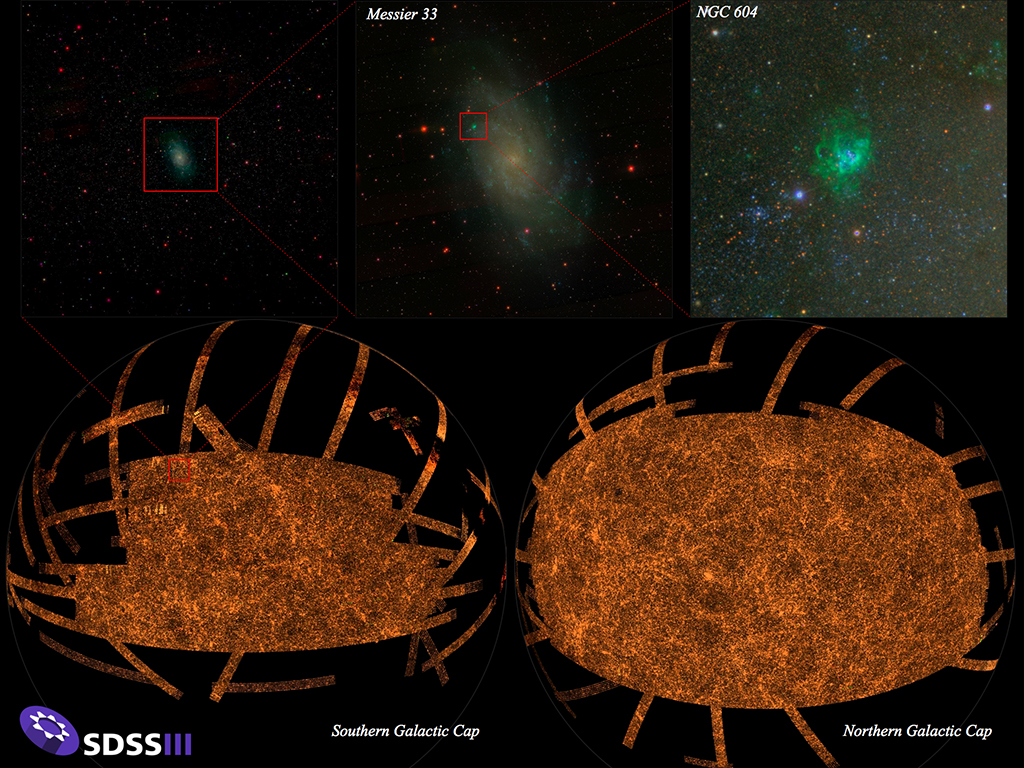
\includegraphics[width=\linewidth]{orangespider-smaller.jpg}
    \caption{Regiones del cielo cubiertas por el catálogo SDSS.}
    \label{fig:sky_araña}
\end{figure}
SDSS trabaja con 5 filtros llamados u,g,r,i,z; es normal caracterizar a las galaxias según sus características en el filtro r ya que es el que se asemeja mas a la región visible del especctro electromagnético

En este trabajo se utiliza una muestra de 20000 galaxias que forman parte del catálogo DR17 de SDSS \citep{2022ApJS..259...35A}, de las cuales se realizo una limpieza preliminar y se uso los datos fotométricos y espectroscópicos de los mismos.
Para este tipo de 

Por 

\subsection{Muestras de galaxias}
Tenemos como proposito trabajar con las propiedades generales de las galaxias por tanto queremos trabajar con un conjunto de muestra que sea grande, arbitrario y uniforme. Ahora esto último se complica al tener en cuenta que el universo esta en expansión y en como esto afecta a la radiación que nos llega de cada galaxia, teniendo esto en cuenta podemos definir dos tipos de muestras: \textbf{muestras completas por flujo} y \textbf{muestras compllets por volumen}

\begin{itemize}
\item
\item
\end{itemize}

Mas adelante detallaremos en cual categoria entra nuestra muestra de datos.

\section{Marco teórico}
Esta sección pretende ser una versión resumida de los conceptos y características a usar en este trabajo, tratando de enfocarse en las definiciones utilizadas por SDSS para luego utilizar en los resultados y discusiones.

\subsection{Morfología de una galaxia}
La característica más básica de cualquier objeto es su forma, para una galaxia esto no es distinto, por tanto a lo largo del tiempo se han desarrollado distintos métodos para clasificar las galaxias según su forma y que diferencias existen entre una y otra.
Hoy en dia la mas utilizada es  aquella desarrollada por Hubble a principios del siglo XX \citep{1926ApJ....64..321H}, en esta se clasifica a las galaxias en 4 tipos generales: \textbf{elípticas, espirales, lenticulares e irregulares}


\begin{itemize}
    \item \textbf{Galaxias elípticas (E)} son galaxias que tienen isofotas\footnote{Las isofotas son contornos a lo largo de los cuales el brillo superficial de una fuente es constante. Si el perfil de luz de una galaxia es elíptico, entonces sus isofotas son elipses.} casi elípticas sin ninguna estructura claramente definida. Se subdividen según su elipticidad $e = 1 - b/a$, donde $a$ y $b$ denotan los semiejes mayor y menor, respectivamente. Las elípticas se encuentran en un rango relativamente amplio de elipticidad, $0 \lesssim e\lesssim 0.7$. La notación E$n$ se utiliza comúnmente para clasificar las elípticas con respecto a $e$, con $n = 10(1 - b/a)$; es decir, una galaxia E4 tiene una relación de ejes de $b/a = 0.6$, y las E0 tienen isofotas circulares. En términos de población estelar se sabe que las elípticas suelen tener la menor tasa de formación estelar y la población que posee suele ser una población vieja.

    \item \textbf{Galaxias espirales} consisten en un disco con estructura de brazos espirales y un bulbo central. Se dividen en dos subclases: espirales normales (S) y espirales barradas (SB). En cada una de estas subclases, se define una secuencia ordenada según la relación de brillo entre el bulbo y el disco, denotada por a, ab, b, bc, c, cd, d. Tienen una población estelar mas compleja, el disco suele ser tener una población más joven y concentra la formación estelar de la galaxia, mientras que el halo suele contener a las estrellas más viejas y enrojecidas.

    \item \textbf{Galaxias irregulares (Irr)} son galaxias con solo estructura regular débil (Irr I) o sin estructura regular (Irr II). Son las que presentan mayor tasa de formación estelar, tanto así que a veces se las suelen confundir con regiones formadoras de estrellas de nuestra galaxia. También entran en esta categoría aquellas galaxias que se encuentran interactuando entre sí y que por lo tanto estan en proceso de cambiar su morfología.

    \item \textbf{Galaxias S0} son una transición entre elípticas y espirales que también se llaman \textit{lenticulares} por su forma de lente. Contienen un bulbo y una gran región envolvente de brillo relativamente no estructurado que a menudo aparece como un disco sin brazos espirales.
\end{itemize}

Cuando Hubble creo esta clasificación la penso como una clasificación evolutiva, donde las elípticas eran las galaxias más jovenes o \textit{tempranas} y las espirales las mas evolucionadas o \textit{tardías}, hoy en día se sabe que esto no es así pero los nombres \textit{tempranas} y \textit{tardías} se siguen usando con frecuencia; este trabajo no es la exccepción, también mencionaremos a estos tipos para diferenciar a las galaxias en ciertas ocasiones.


\subsection{Tamaño de una galaxia}
Definir el tamaño de una galaxia es una tarea delicada, en parte por que hay que definir para una dada imagen hasta donde llega la galaxia y en parte por que una misma galaxia puede presentar distintos tamaños en distintos filtros, por tanto no es un parámetro que este univocamente definido sino que es necesario llegar a un término intermedio que pueda resultar útil para todas las galaxias. 
SDSS logra esto definiendo su tamaño como el radio dentro del cual se concentra un cierto porcentaje del brillo total de la galaxia. \\
En general son parámetros típicos $r_{50}$, el radio que contiene el $50\%$ del flujo total, y $r_{90}$ en el cual se concentra el $90\%$.


\subsubsection{Parámetro de concentración}
Es un parámetro que marca que tan concentrada es un galaxia
Se define como:
\begin{equation}
	C=r_{50}/r_{90}
\end{equation}

\subsection{Magnitudes}
Las magnitudes son la característica más básica de cualquier objeto astronómico, nos dice cuanta luz emite y permite inferir mucha info. Pero para poder calcularla necesitamos poder definirla, para un objeto puntual, como una estrella, esta definición es sencilla, pero para un objeto extenso, como una galaxia, esta definición resulta mas complicada ya que para definirla correctamente hay que definir que región es parte de la galaxia y que región no.
Es en estos casos que la definicion de la característica depende de como la defina el catálogo, en el caso de Sloan se definen distintos tipos de  magnitudes para cada filtro, pero en particular nos centramos en: \textbf{magnitud model} y \textbf{magnitud petro}, .

\subsubsection{Magnitud model}
Una vez extraida la dsitribución de brillo de la galaxia se ajustan por separado dos módelos de dsitribución de brillo:
\begin{itemize}
	\item Perfil de De Vaucouleurs \citep{1948AnAp...11..247D}: \[I(r) = I_0 e^{-7.67 [(r/re)1/4]} \]
	\item Perfil exponencial \citep{1970ApJ...160..811F}: \[I(r) = I_0 e^{-1.68r/re}\]
\end{itemize}
Una vez ajustado cada uno se compara la bondad del ajuste en cada caso y se define a la magnitud model usando la Ley de Pogson: 


\begin{equation}
m_{model}= [22.5 \text{mag}] - 2.5 log_{10} (f)
\end{equation}

Definirse a partir de un perfil teórico tiene sus ventajas y desventajas, por un lado no dependen de un radio donde exista la galaxia por tanto es la magnitud ideal para medir índices de color, pero por otro lado tiene el problema de que no todas las galaxias siguen puramente uno u otro módelo como sabemos gracias a la Ley de Sérsic \citep{1963BAAA....6...41S}, por tanto no siempre ajusta bien.
Los flujos medidos en cada filtro son hechos con anchos equivalentes para que los indices de color queden bien definidos

\subsubsection{Magnitud petrosiana}
Se definen usando To satisfy these requirements, the SDSS has adopted a modified form of the Petrosian (1976) system, measuring galaxy fluxes within a circular aperture whose radius is defined by the shape of the azimuthally averaged light profile.

In the SDSS five-band photometry, the aperture in all bands is set by the profile of the galaxy in the r band alone. This procedure ensures that the color measured by comparing the Petrosian flux FP in different bands is measured through a consistent aperture.


\subsubsection{Parámetro fracDeV}
SDSS define un 3er tipo de magnitud que no se utilizó en este trabajo pero que dio pie a la definición del parámetro fracDeV dentro del catálogo; las \textit{Composite Model Magnitudes} o magnitudes módelo compuestas se definen con los mismos perfiles que las magnitudes módelo solo que en vez de elegir solamente 1 se las define como una combinación lineal pesada de ambos: \[F_{\text{composite}} = fracDeV \,FdeV + (1 - fracDeV)\,Fexp\]. 
Por tanto $fraDeV$ es un parámetro en el cual se cuantiza que ``tanto'' se asemeja el pérfil de brillo respecto al pérfil de la ley de De Vaucoulers.\\
Este parámetro sirve como un primer \textit{approach} para conocer la componente principal de una galaxia, en este trabajo en específico se tomó que si $fracDeV \leq 0.2$ entonces el disco es prominente mientras que si $fracDeV \geq 0.8$ el bulbo es mas prominente.



\subsection{Brillo superficial}
El brillo superficial es simplemente un parámetro que nos dice la cantidad de flujo de radiación por unidad de superficie que recibimos de un objeto. Para el caso de una galaxia resulta de interés ya que 
\cite{2005PASA...22..118G}


\section{Datos}
Se descargaron 20000 galaxias usando la pagina CasJobs, de este se descargaron las siguientes columnas de las tablas Galaxy y SpecObj con los limites ($0.02,0.05$)  para el redshift y ($14,18$) para la magnitud petrosiana r desafectada por la extinción interestelar de la Vía Láctea.
Las restricciones a la magnitud se hicieron por 2 motivos principales: 
\begin{itemize}
\item La sensibilidad del espectrógrafo de SDSS nos asegura una completitud de la muestra hasta $m_r\sim17.77$ mas alla de este punto no se asegura que se haya obtenido un espectro confiable de la galaxia
\item Si una galaxia es muy brillante $m_r\sim14$ entonces hay mas probabilidades de que la imagen que toma la fibra se sature y no se pueda obtener un espectro de utilidad. 
\end{itemize}
 
 Ademas se agrego otra 

Como analisis preliminar se realizo el diagrama \ref{fig:araña}, donde ubicamos las galaxias en el cielo donde se comprueba que la muestra este distribuida uniformemente en el cielo y no exista una sobredensidad en el cielo.



\begin{figure}[ht]
    \centering
    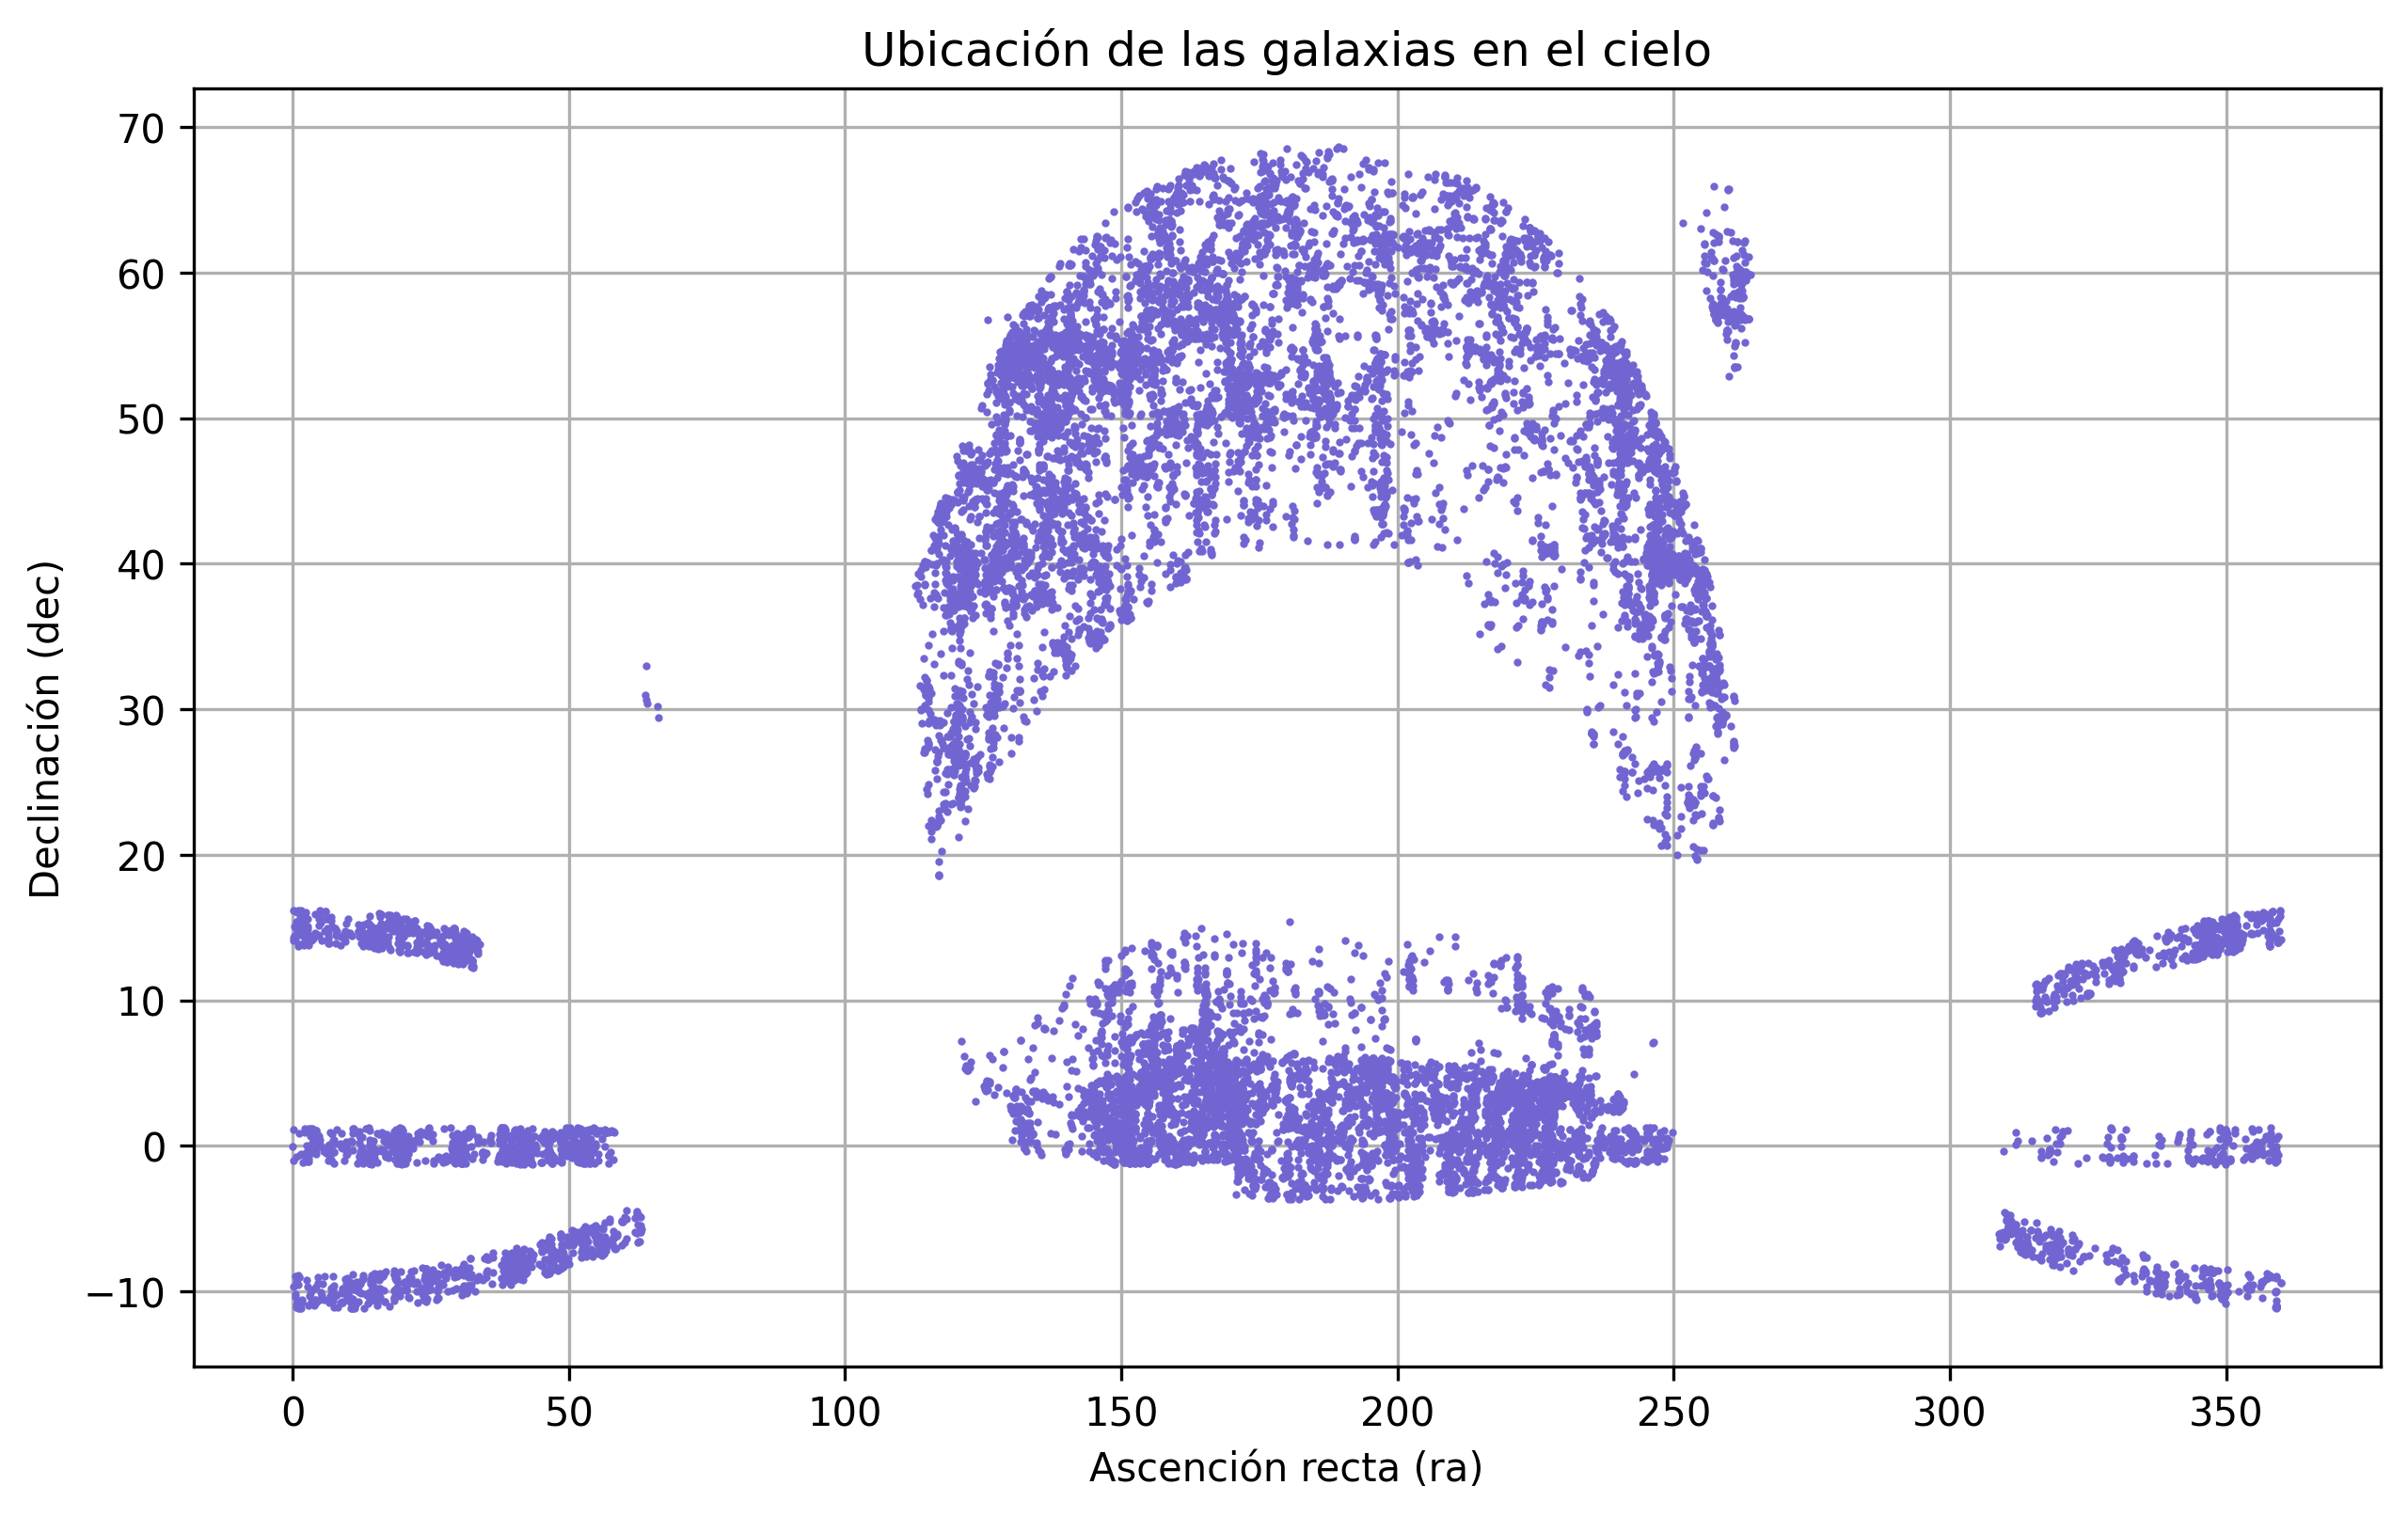
\includegraphics[width=\linewidth]{gal_in_sky.png}
    \caption{Ubicación en el cielo de las galaxias seleccionadas.}
    \label{fig:araña}
\end{figure}

También se realizo el diagrama \ref{fig:hist_z} para comprobar la distribución del redshift de las galaxias, podemos ver que 

\begin{figure}[ht]
    \centering
    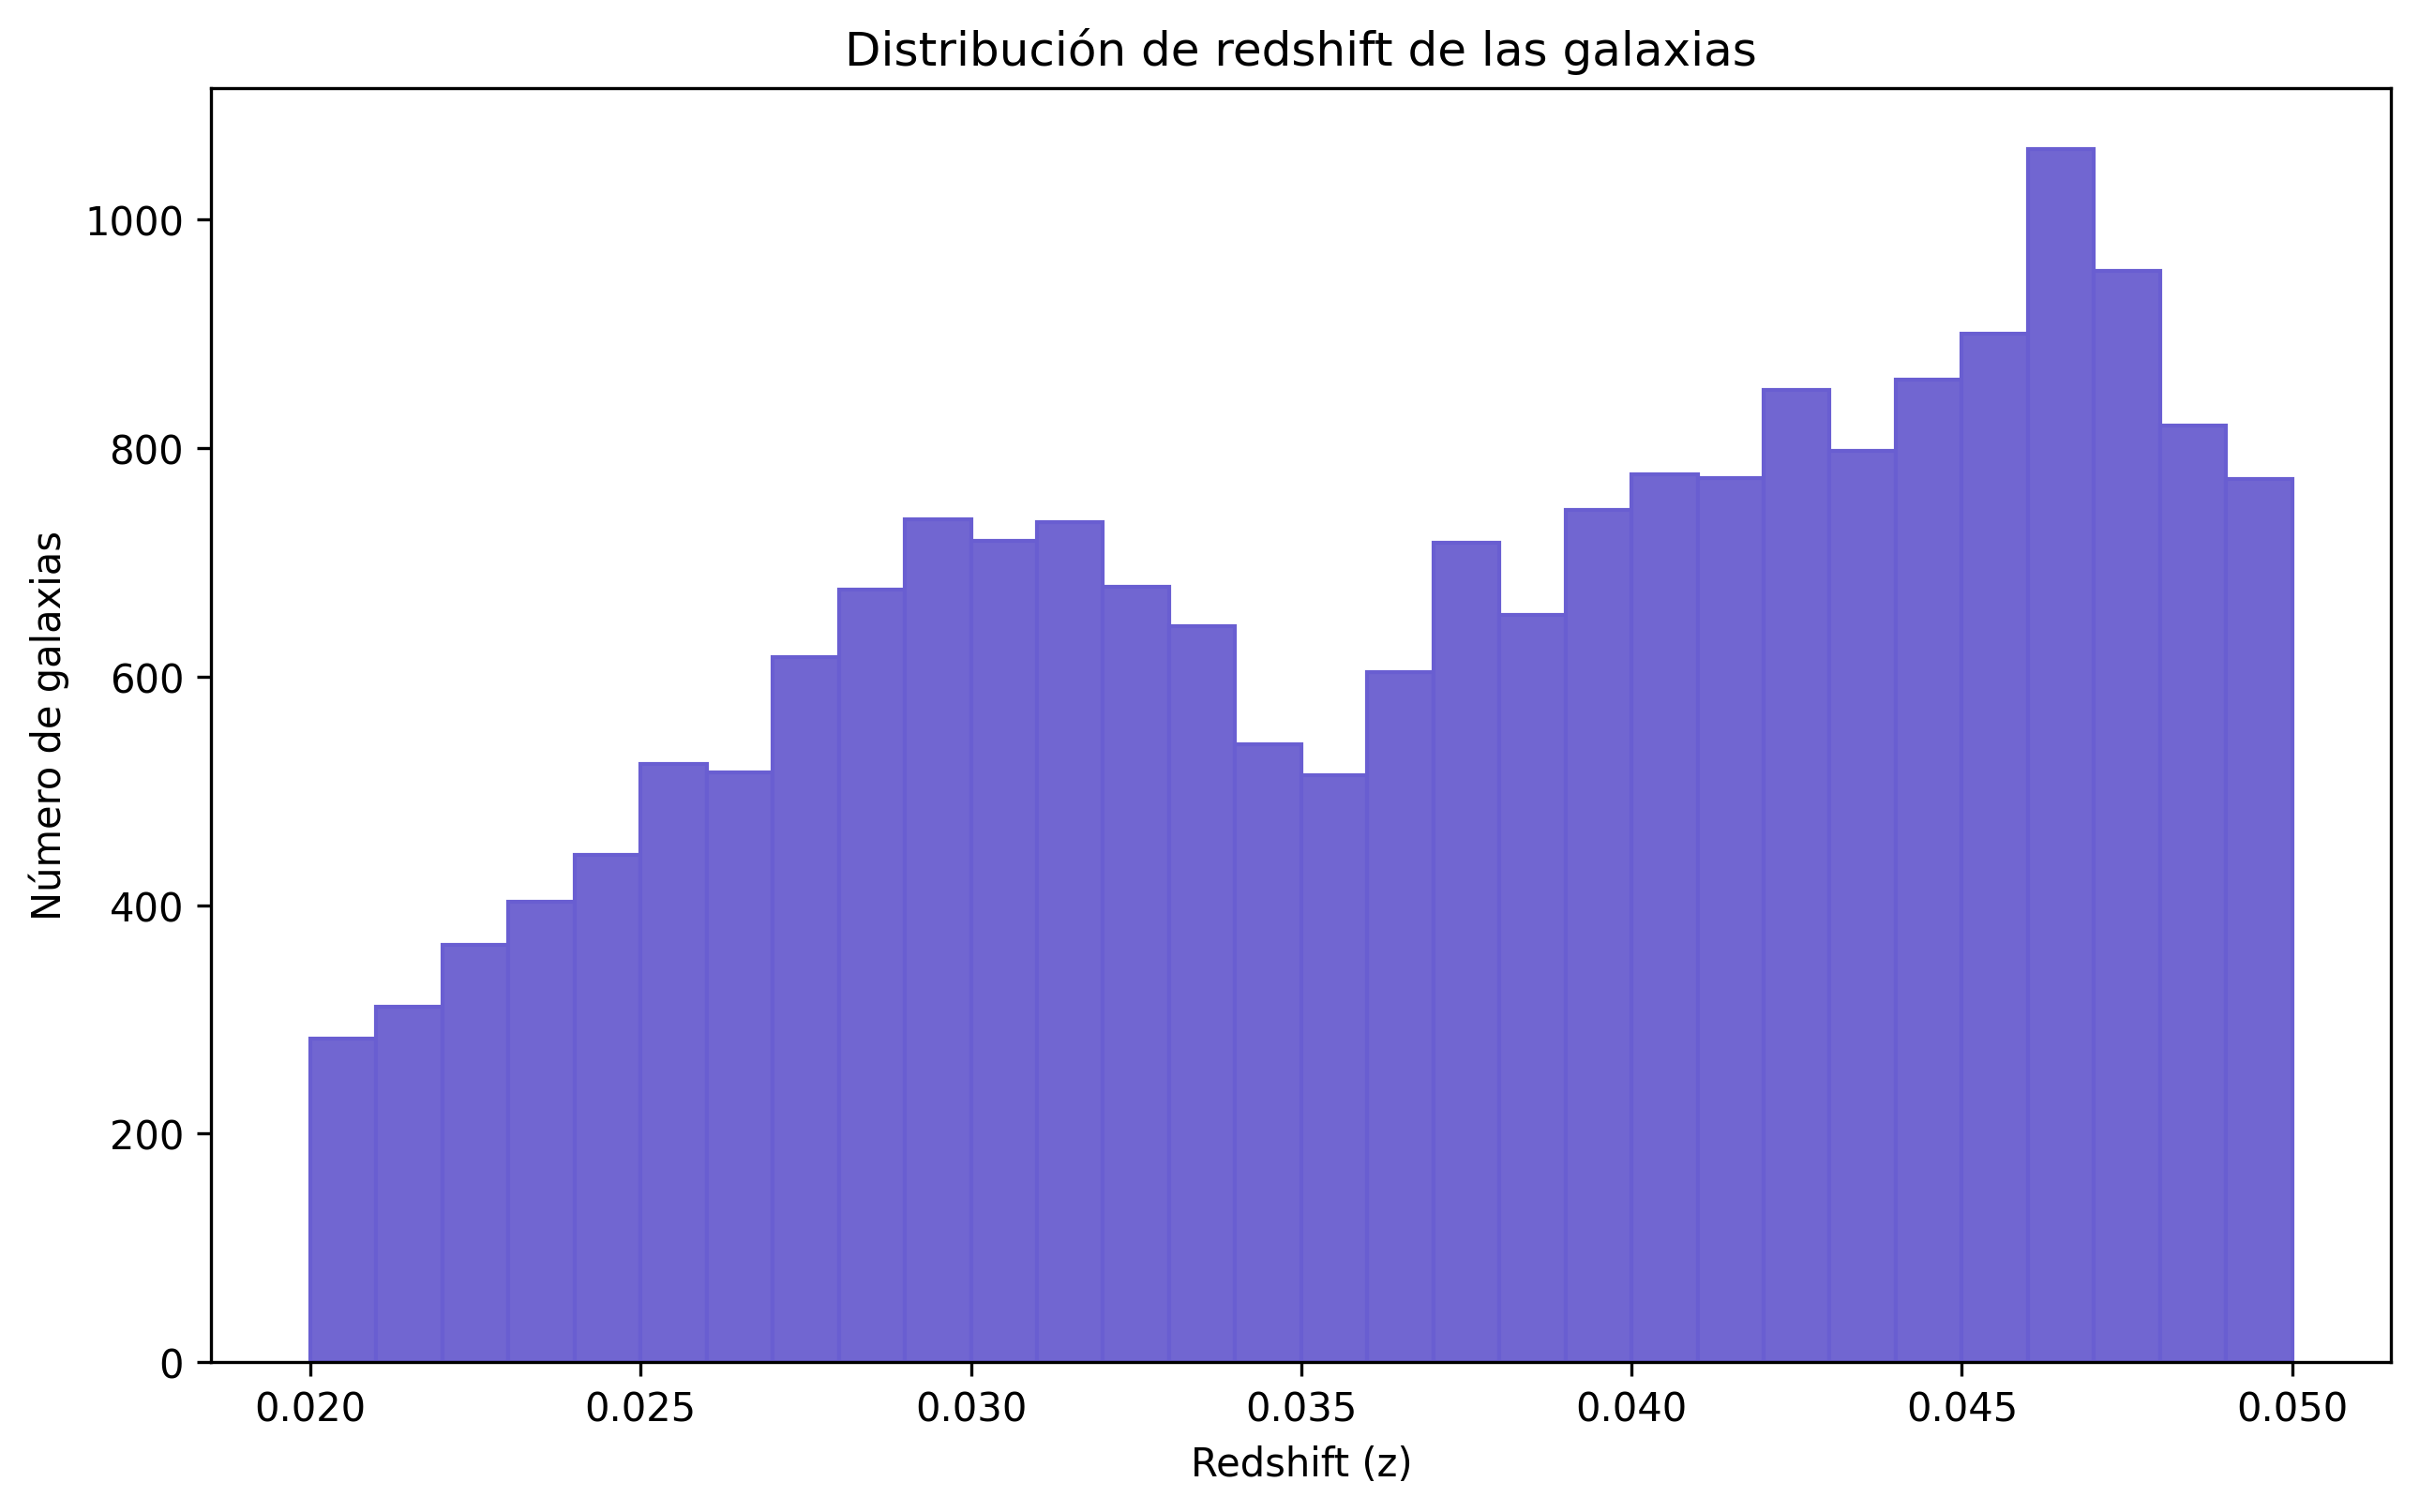
\includegraphics[width=\linewidth]{gal_z.png}
    \caption{Ubicación en el cielo de las galaxias seleccionadas.}
    \label{fig:hist_z}
\end{figure}


En el diagrama \ref{fig:completo_flujo} se grafica ... para ver la distribucion de la magnitud aparente, vemos que el conjunto obtenido es lo que se denomina una muestra completa por flujo, es decir que las muestras se distribuyen uniformemente a lo largo de un rango de magnitudes.
\begin{figure}[ht]
    \centering
    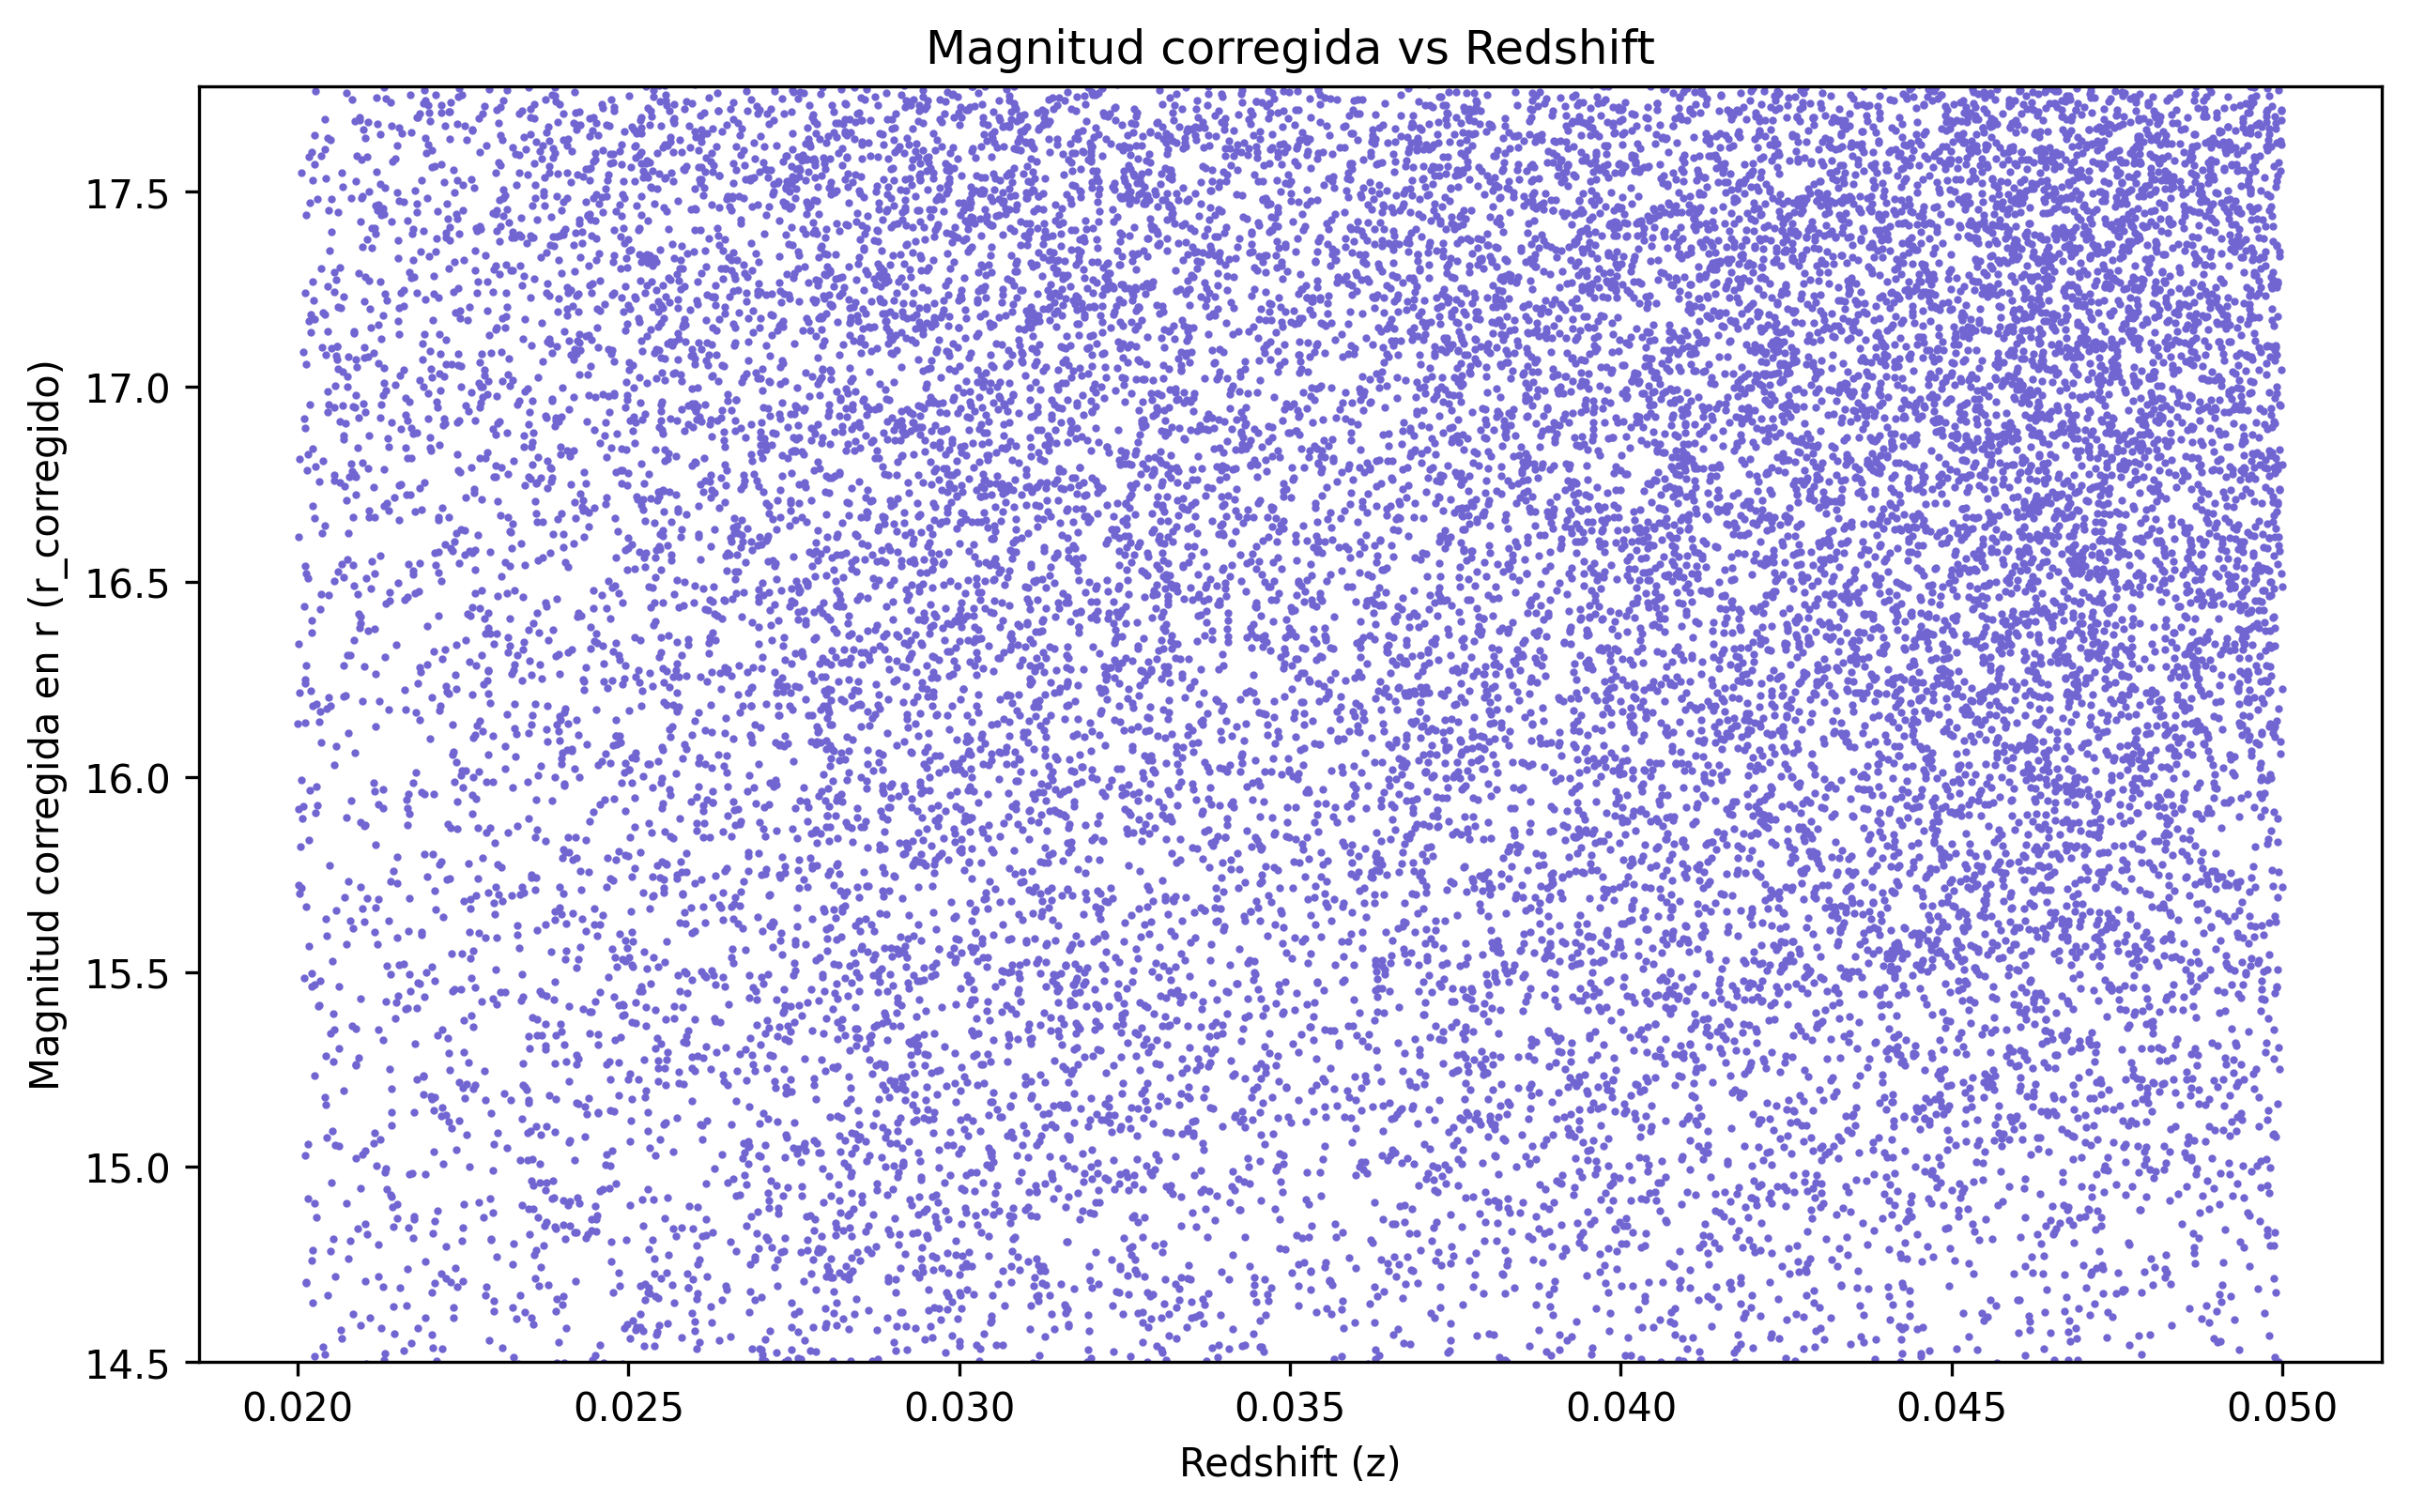
\includegraphics[width=\linewidth]{mag_vs_z.png}
    \caption{Ubicación en el cielo de las galaxias seleccionadas.}
    \label{fig:completo_flujo}
\end{figure}


\section{Resultados y discusiones}

\subsection{Magnitud absoluta}
Usando el $z$ de cada galaxia y eligiendo $H_0=70 Mpc^{-2}$, $\Omega_{mat}=0.3$, $\Omega_{\Lambda}=0.7$ como cosmología podemos calcular la distancia luminosa de la galaxia, la cual por definición nos permite usarla para calcular la magnitud absoluta de la galaxia teniendo en cuenta los efectos debidos a la expansión del universo.

\begin{equation}
d_L=(1 + z)\frac{c}{H_0} \int_0^z \frac{dz'}{\sqrt{\Omega_m(1+z')^3 + \Omega_\Lambda \quad \left[d_L\right]=Mpc
\end{equation}

De la ecuación del módulo de la distancia y usando las correcciones AB para llevarlo al sistema módelo llego a la siguiente ecuación para la magnitud absoluta:
\begin{equation}
M_i = m_i - ext_i + corr-ab_i - 5log_{10}(d_L) -25
\end{equation}

Donde \[i=\left(u,g,r,i,z \right) \] los filtros disponibles en Sloan. Al hacer estas correcciones podemos repetir lo visto en la figura \ref{fig:completo_flujo} pero con la magnitud absoluta en la figura \ref{fig:M_r_hist}

\begin{figure}[ht]
    \centering
    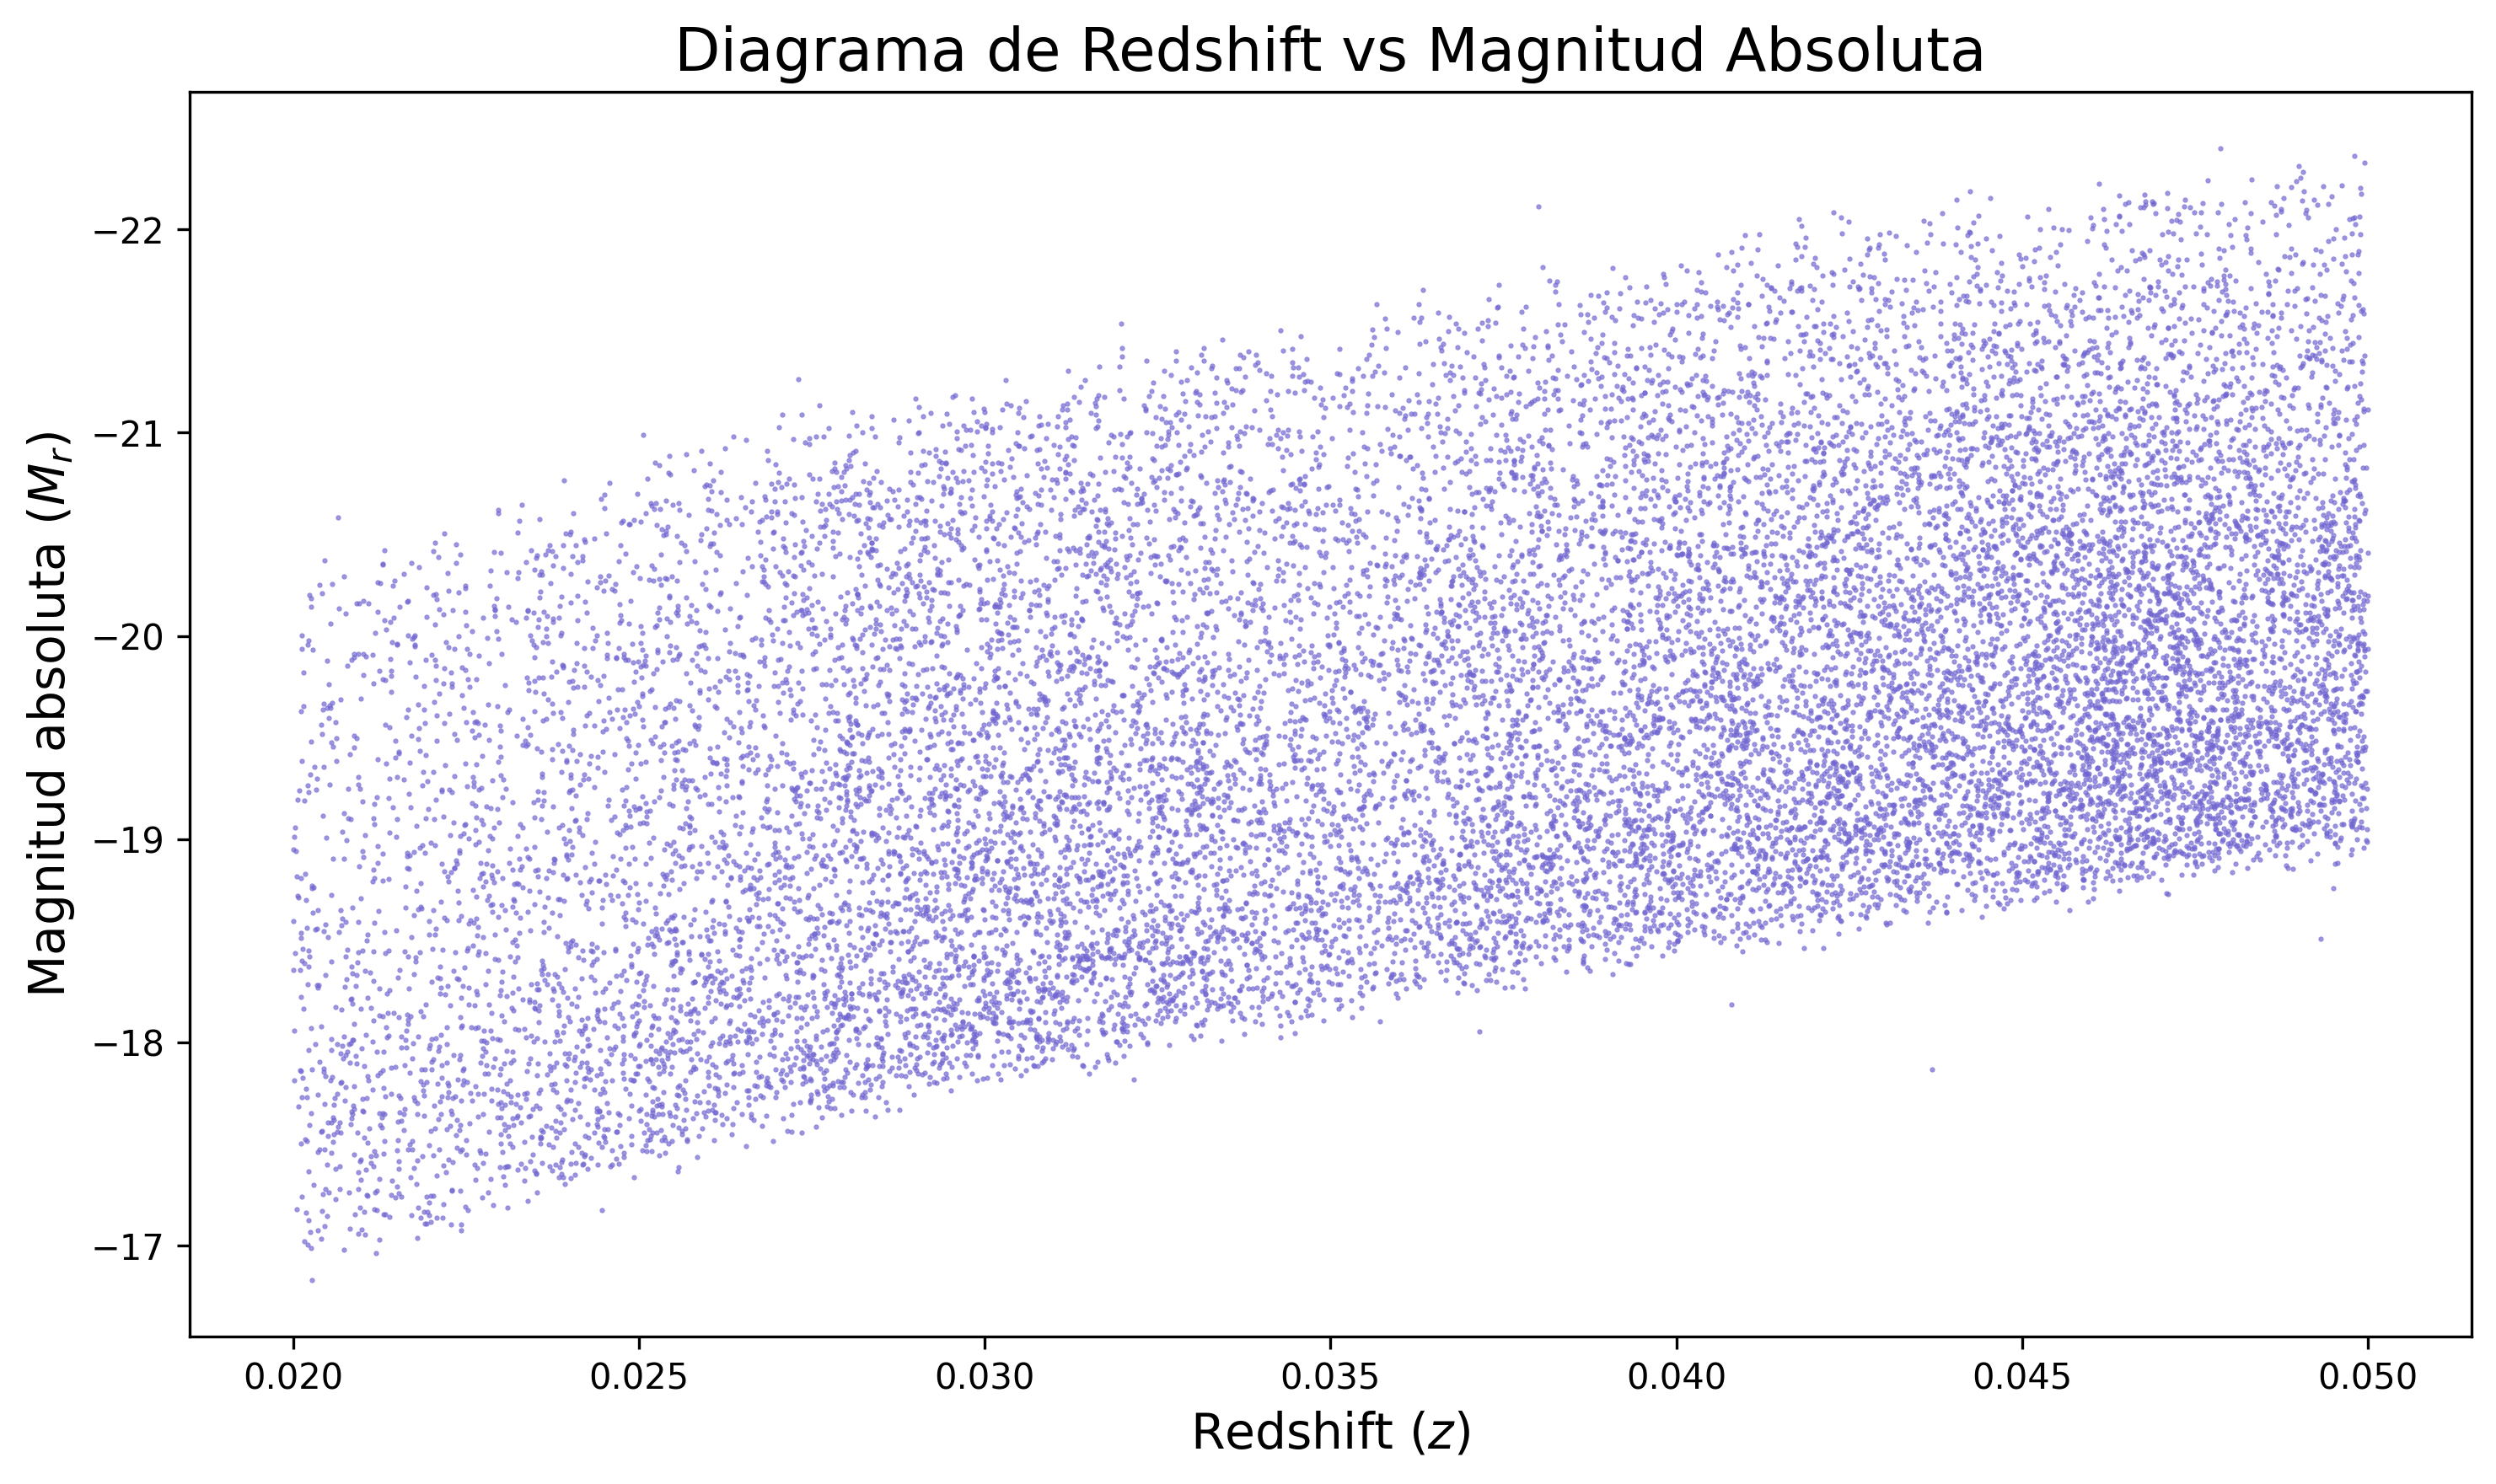
\includegraphics[width=\linewidth]{mabs_vs_z.png}
    \caption{Ubicación en el cielo de las galaxias seleccionadas.}
    \label{fig:M_r_hist}
\end{figure}

Con la figura \ref{fig:M_r_hist} podemos ver que la muestra ccon la que estamos trabajando no es completa en volumen ya que la distribución de las galaxias varia con el redshift (a mayor $z$ menor magnitud absoluta, es decir vamos perdiendo a las galaxias menos brillantes), ademas que lo que antes se veía como un bloque uniforme ahora se nota como en con la magnitud absoluta pasa a seguir una forma mas logaritmica debido a la dependencia de $M_r$ respecto de la distancia luminosa y por tanto del $z$.



\subsection{Índices de color}
Los índices de color son una de las herramientas mas útiles de cualquier astrónomo, en particular sabemos por \cite{2004ApJ...600..681B} que las galaxias tienen un rango de ($0,4$) para el índice $u-r$ y de ($0,1$) para el índice $g-r$, ademas presentan una  cierta bimodalidad, características que se observan claramente en la figura \ref{fig:colores}, con esto en mente podemos clasificar a las galaxias como rojas o azules. 

Para separar por color se ajusto dos distribuciones gaussianas al índice u-r, ya que es donde el cambio es más marcado debido a una mayor diferencia entre las longitudes de onda de cada filtro, y se selecciono como límite el punto donde ambas gaussianas se tocan, esto es en el punto $u-r \sim 2.10$. Con esto se separon a las galaxias según su color como se muestra en la figura \ref{fig:red_blue}

\begin{figure}[ht]
    \centering
    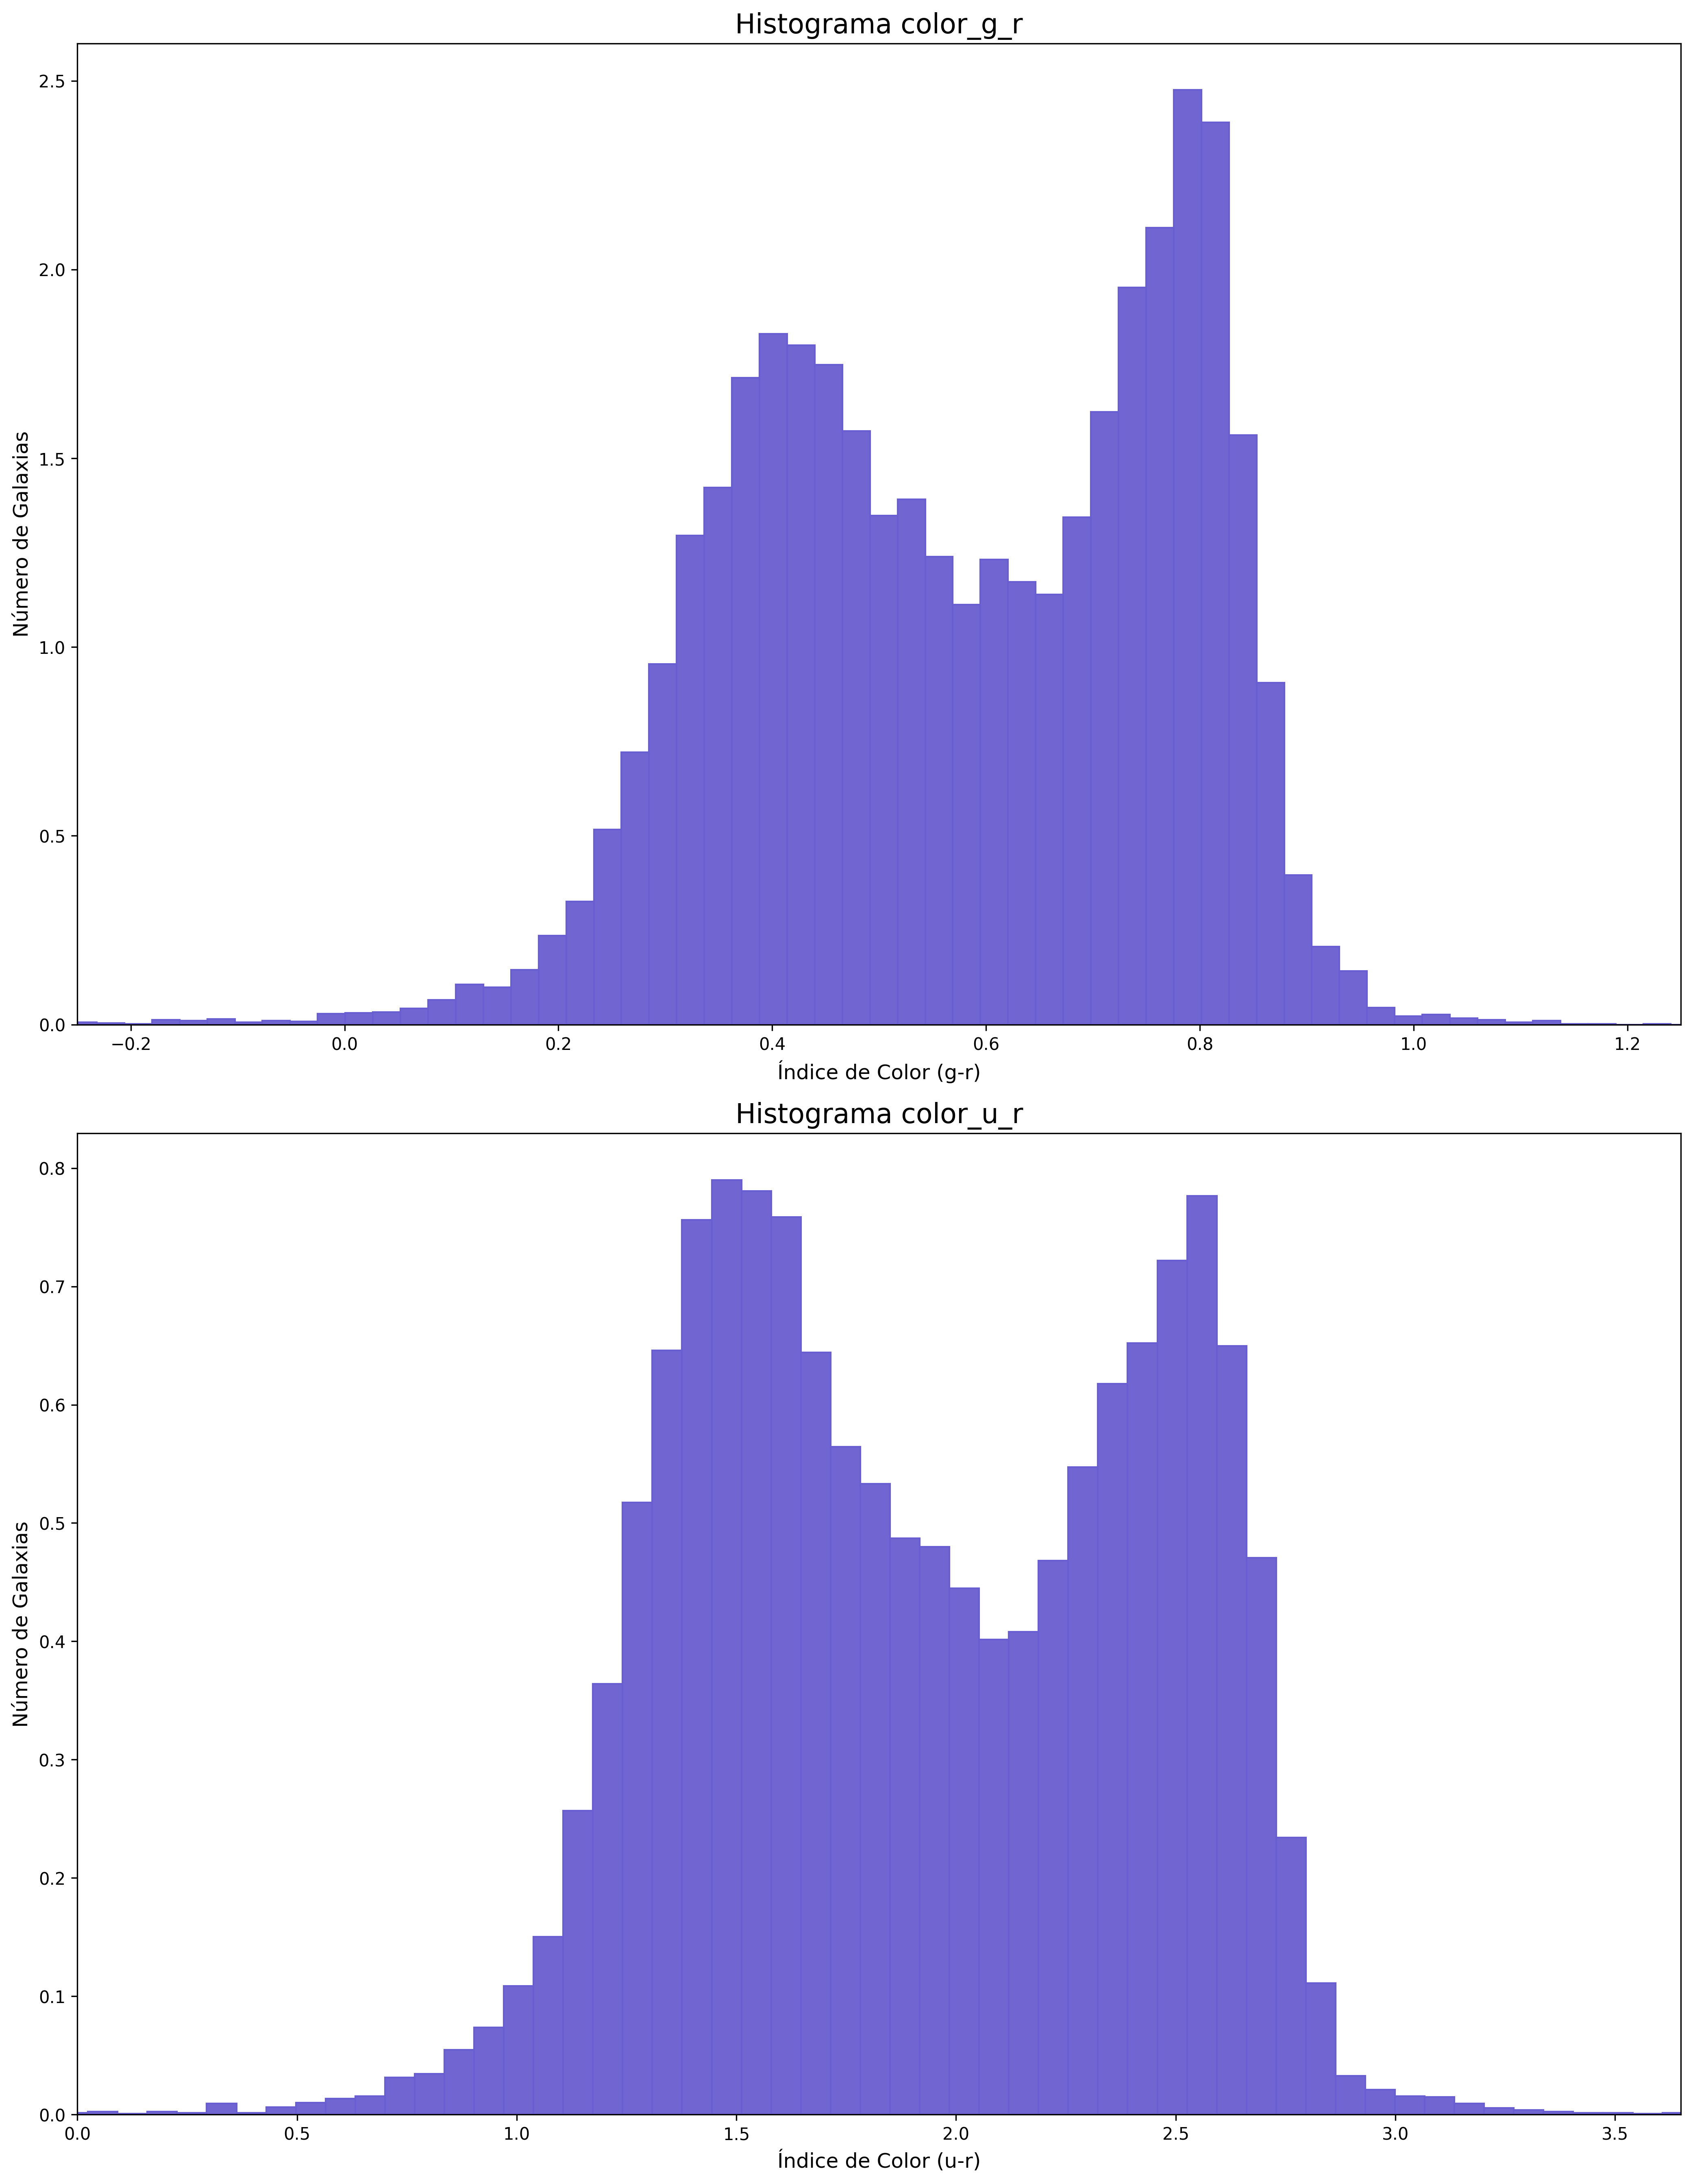
\includegraphics[width=\linewidth]{colores.png}
    \caption{Histograma de los índices de color de las galaxias seleccionadas.}
    \label{fig:colores}
\end{figure}

\begin{figure}[ht]
    \centering
    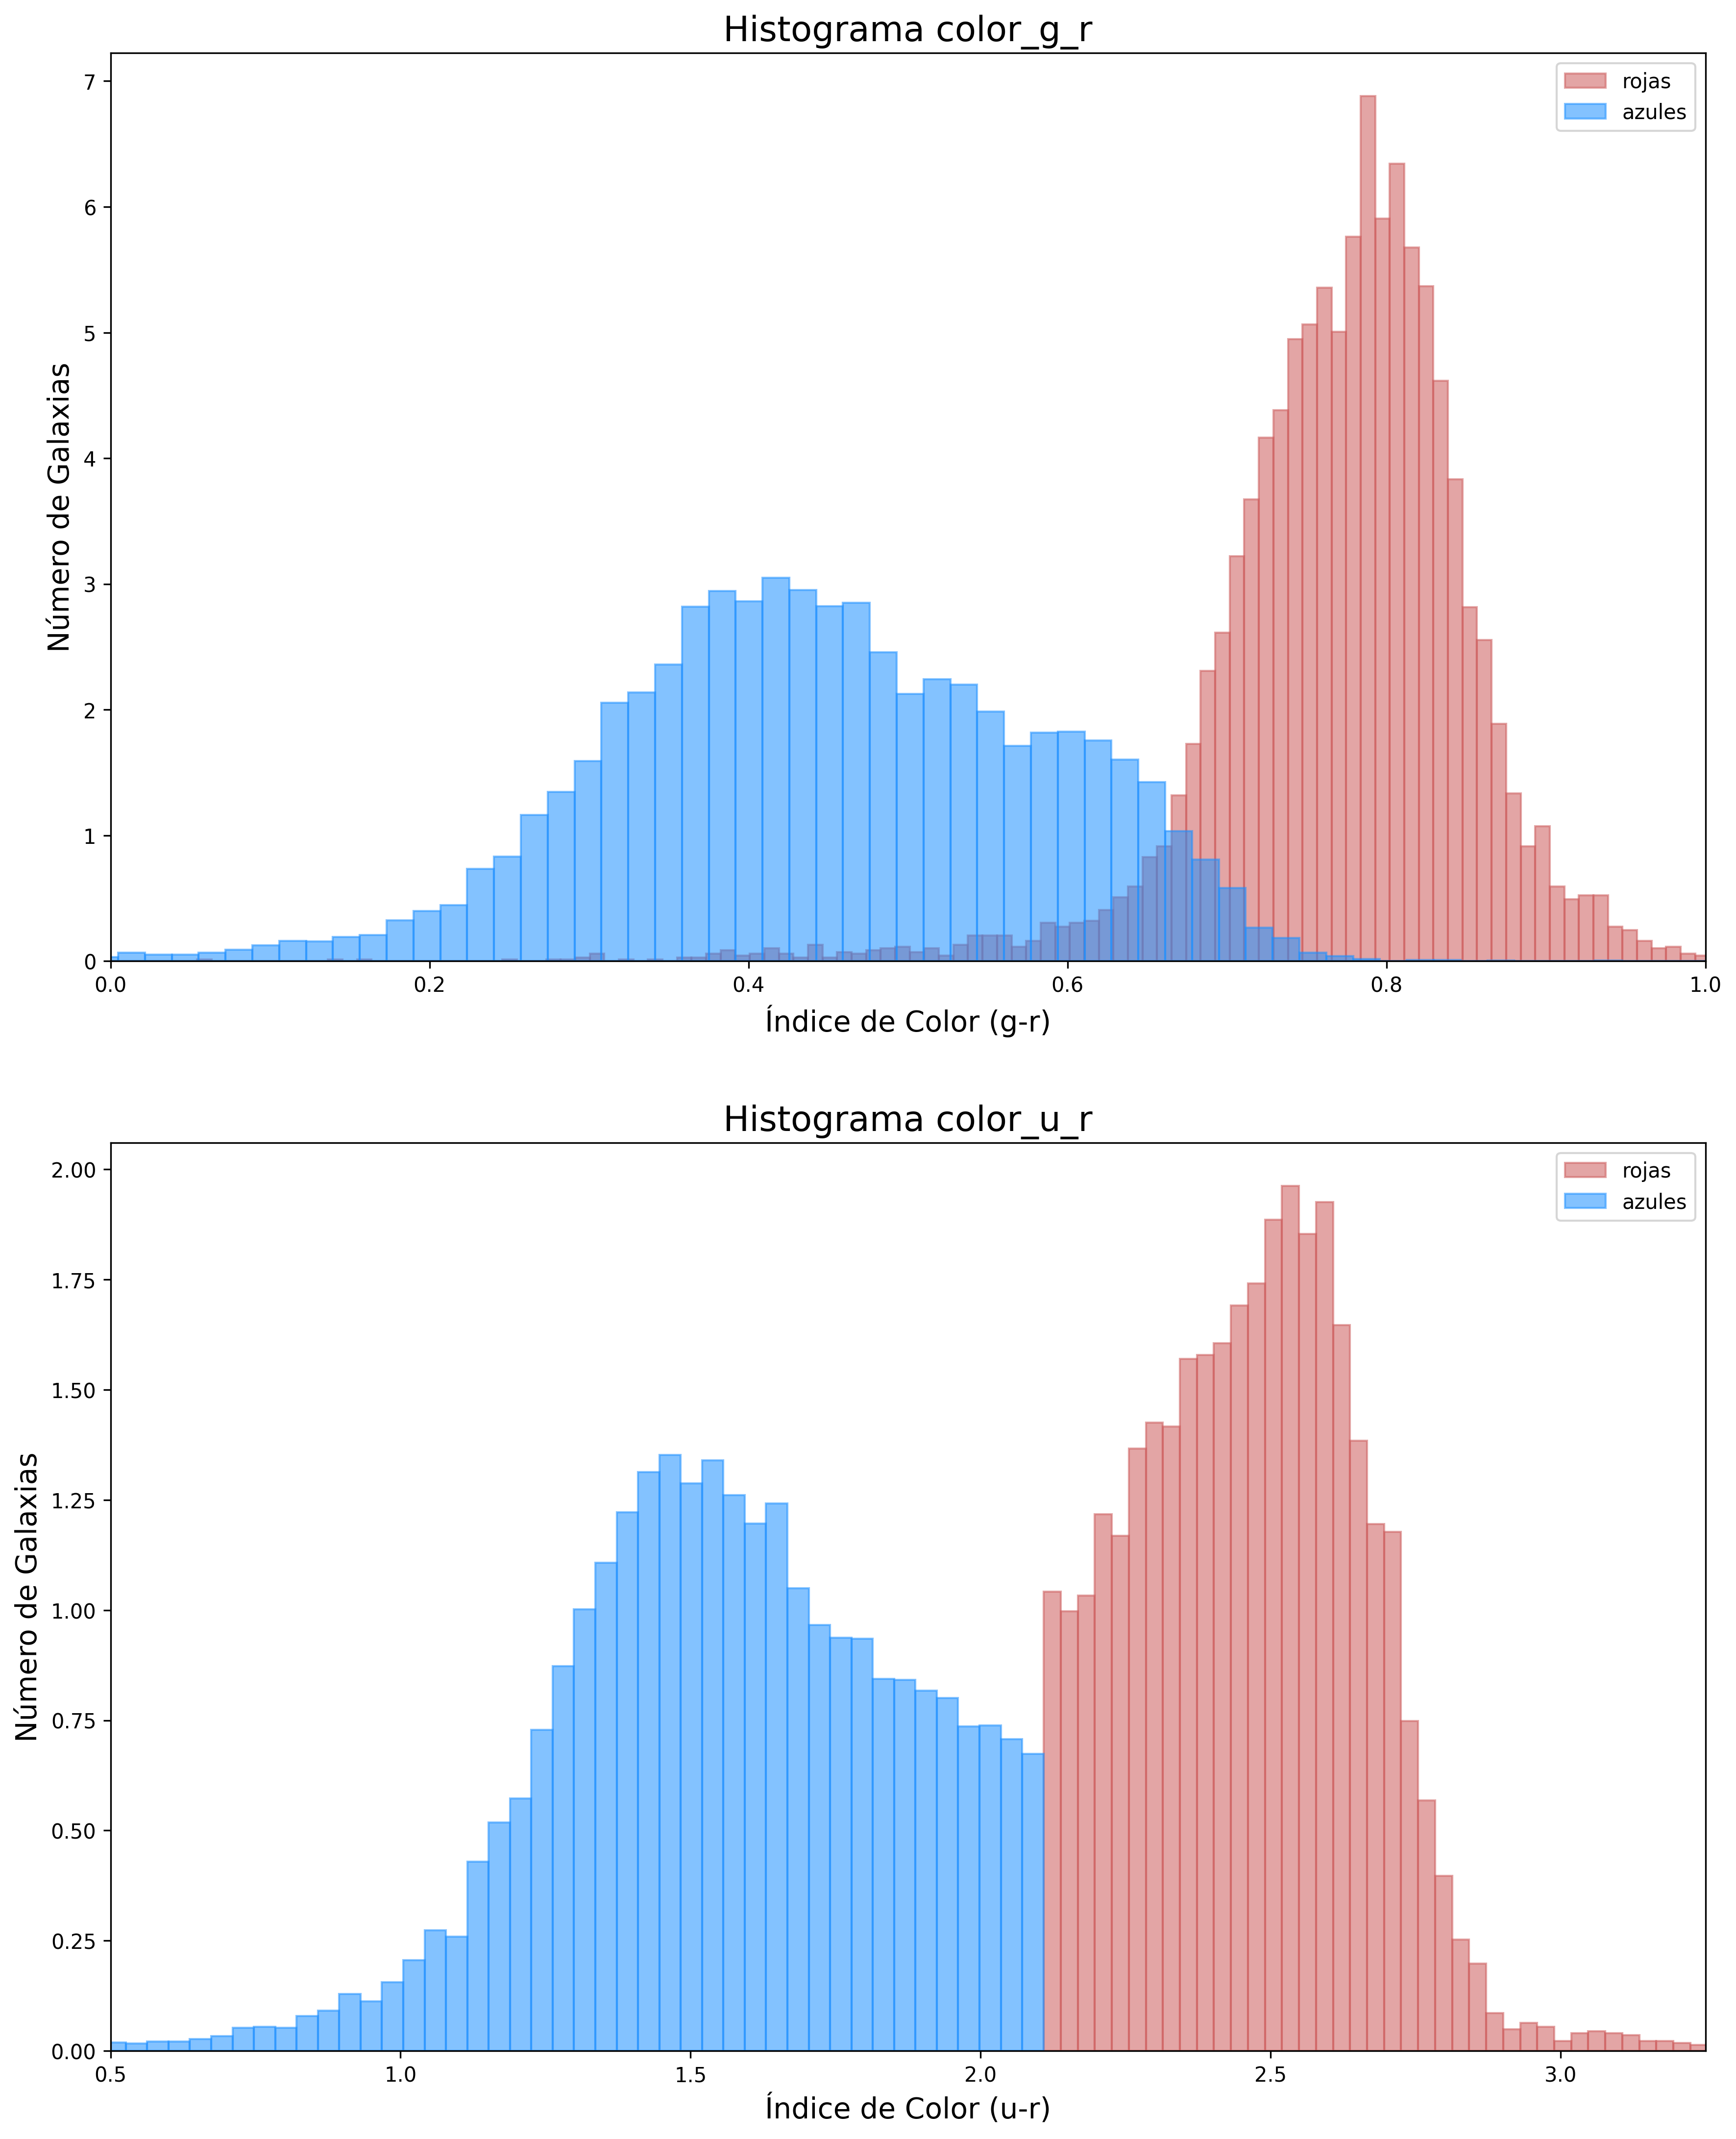
\includegraphics[width=\linewidth]{rojas_y_azules.png}
    \caption{Histograma de los índices de color de las galaxias  rojas y azules.}
    \label{fig:red_blue}
\end{figure}



\subsection{Brillo superficial}

\section{Conclusiones}
\subsection{Clasificación}






\bibliographystyle{plainnat}
\bibliography{bibliografia}

\end{document}
